\section{CHAPTER 7: BOILERS}
\subsection{Acquaintance}
Boilers are integral components of modern industrial processes and residential heating systems, designed to convert water into steam or hot water using various fuel sources such as natural gas, oil, coal, or electricity. This thermal energy is then utilized for heating, power generation, and a multitude of other applications. Having evolved from simple fire-tube designs to the advanced and efficient water-tube and electric boilers of today, boilers play a crucial role in multiple sectors, including manufacturing, power generation, and food processing. Their significance lies in their ability to provide consistent and reliable heat and steam, essential for numerous industrial processes. Modern boilers are engineered for greater efficiency, environmental friendliness, and safety, incorporating technologies like condensing capabilities to recover heat from exhaust gases and sophisticated control systems for optimal operation and safety. Understanding the various types of boilers, their components, and operating principles is vital for anyone involved in their maintenance, operation, or design. This report explores the different classifications of boilers, their working mechanisms, and the latest advancements in boiler technology, highlighting their critical role in contemporary industry and daily life.

\begin{figure}[h]
\centering
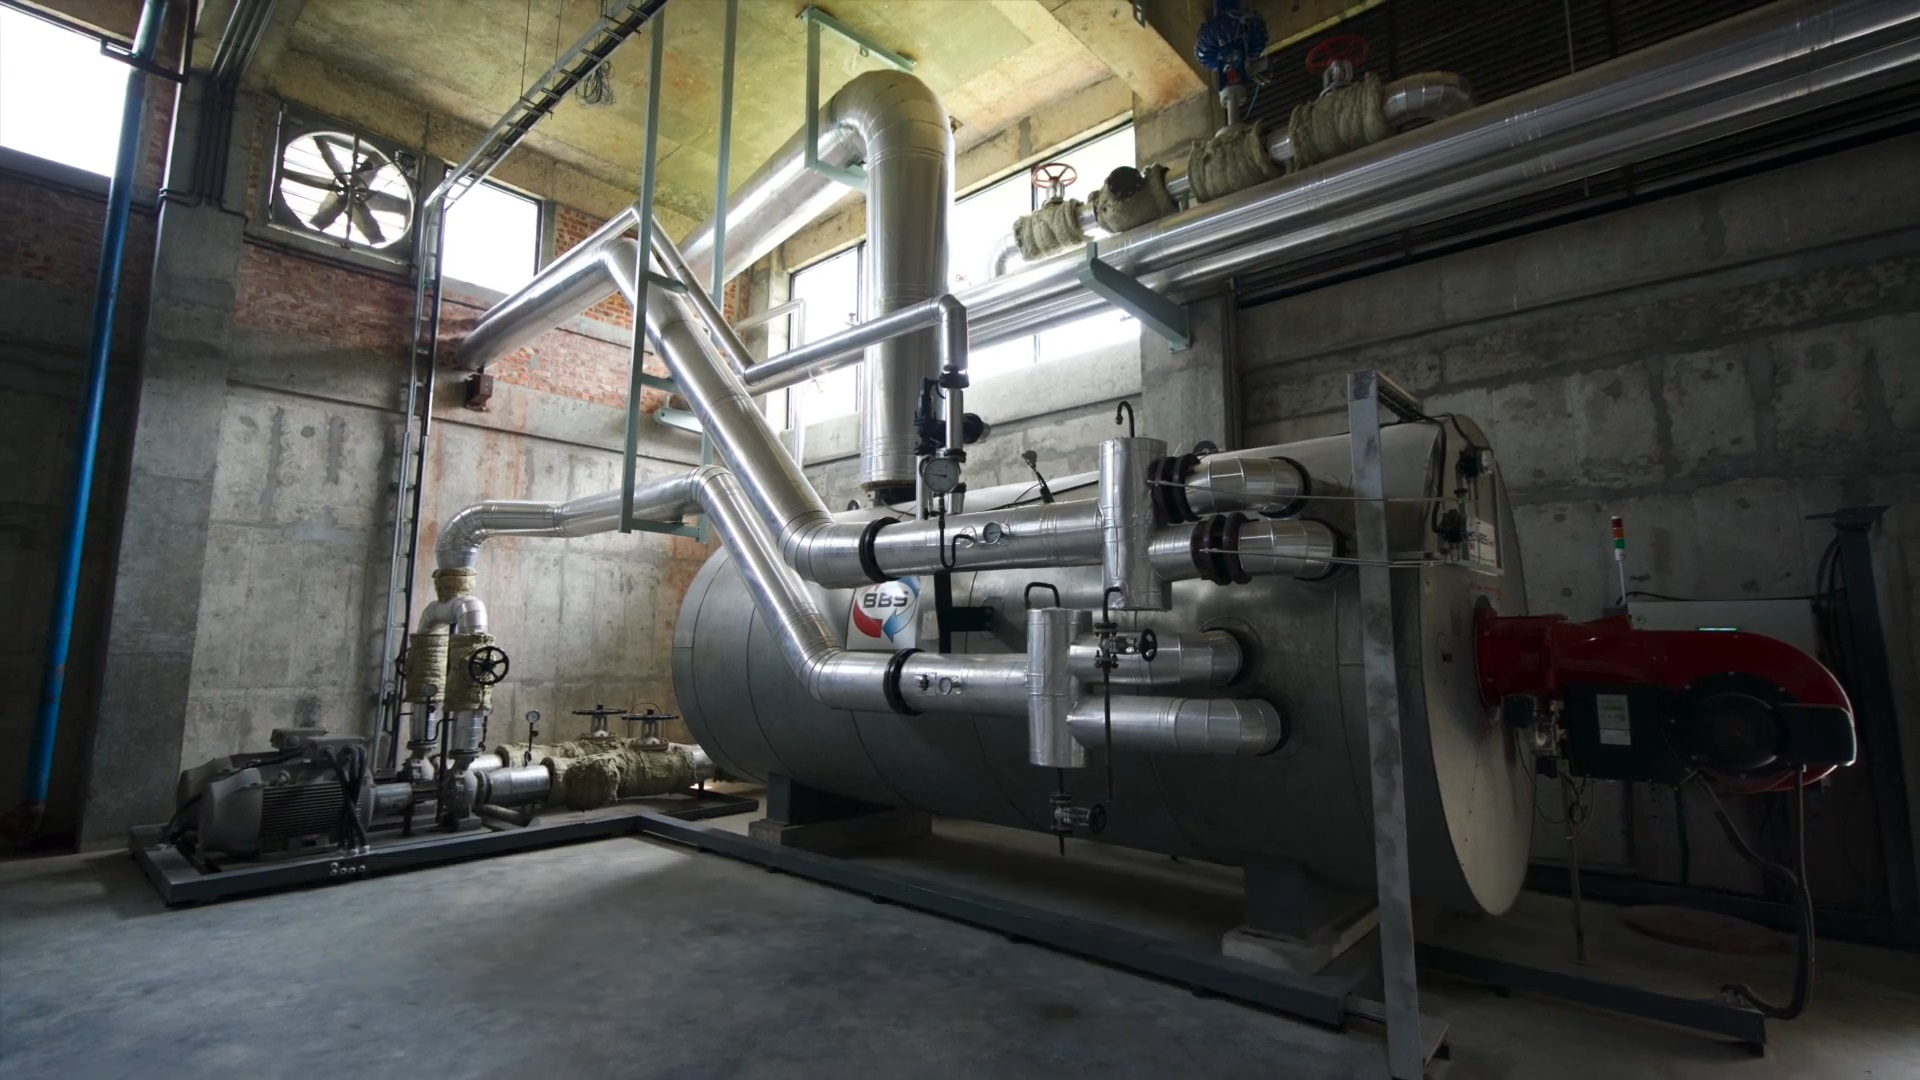
\includegraphics[width=0.8\textwidth]{figs/boiler.jpg}
\caption{Boiler}
\label{fig:boiler}
\end{figure}


\subsection{Types of Boilers}
Boilers can be classified into various categories based on different criteria. Below is a detailed overview of the primary types:

\subsubsection{Based on the position of water and hot gases}
\begin{enumerate}
    \item \textbf{Fire Tube Boiler}: In this type, hot gases pass through tubes surrounded by water.
    \item \textbf{Water Tube Boiler}: Here, water flows through tubes that are heated by external hot gases.
\end{enumerate}

\subsubsection{Based on the position}
\begin{enumerate}
    \item \textbf{External Fired Boiler}: The furnace is outside the boiler shell.
    \item \textbf{Internally Fired Boiler}: The furnace is inside the boiler shell.
\end{enumerate}

\subsubsection{Based on Axis}
\begin{enumerate}
    \item \textbf{Horizontal Boiler}: These boilers have a horizontal axis.
    \item \textbf{Vertical Boiler}: These boilers have a vertical axis.
\end{enumerate}

\subsubsection{Based on Pressure}
\begin{enumerate}
    \item \textbf{Low-Pressure Boiler}: Operates at lower pressures, typically below 15 psi.
    \item \textbf{High-Pressure Boiler}: Operates at pressures above 15 psi.
\end{enumerate}

\subsubsection{Based on the Furnace}
\begin{enumerate}
    \item \textbf{Single Furnace Boiler}: Contains one furnace.
    \item \textbf{Dual Furnace Boiler}: Contains two furnaces.
\end{enumerate}

\subsubsection{Based on the Method of Circulation}
\begin{enumerate}
    \item \textbf{Natural Circulation Boiler}: Water circulates naturally due to convection currents.
    \item \textbf{Forced Circulation Boiler}: Water circulation is forced by a pump.
\end{enumerate}

\subsubsection{Based on Fuel Burning}
\begin{enumerate}
    \item \textbf{Solid Fuel-Fired Boiler}: Uses solid fuels like coal or wood.
    \item \textbf{Oil and Gas Fired Boiler}: Uses oil or gas as fuel.
    \item \textbf{Dual Fired Boiler}: Can use both oil and gas.
    \item \textbf{Exhaust Gas Boiler}: Primarily uses the waste heat from exhaust gases, making them a unique category in terms of fuel usage.
\end{enumerate}

\subsubsection{Based on the Furnace}
\begin{enumerate}
    \item \textbf{Single Furnace Boiler}: Contains one furnace.
    \item \textbf{Dual Furnace Boiler}: Contains two furnaces.
\end{enumerate}


\textbf{Fire-tube Boilers:}
Fire-tube boilers operate by passing hot gases produced from fuel combustion through tubes that are submerged in water. The heat from these gases transfers to the water, generating steam. These boilers are valued for their straightforward design and reliability, making them suitable for various heating applications.

\textbf{Water-Tube Boilers:}
In water-tube boilers, water circulates within the tubes, and these tubes are heated externally by hot gases from the combustion process. This setup allows for higher efficiency and the ability to operate at higher pressures, making water-tube boilers a common choice for power generation and industrial processes.

\textbf{Electric Boilers:}
Electric boilers utilize electricity as their heat source. They contain electric resistance elements to heat the water, making them compact and easy to install. These boilers are often found in residential and commercial settings where traditional fuel sources might not be feasible.

\textbf{Combi Boilers: }
Combination boilers, or combi boilers, are designed to provide both space heating and hot water from a single unit. These boilers are especially popular in residential settings due to their ability to supply hot water on demand, eliminating the need for a separate water heater.

\subsection{Components of a Boiler}
Boilers are complex systems composed of several key components, each serving a specific function to ensure efficient and safe operation. Below is a detailed description of these components:

\begin{enumerate}
    \item \textbf{Furnace Tube}\\
    The furnace tube is where the fuel combustion occurs, generating the necessary heat for the boiler's operation.

    \item \textbf{Tubes (2nd Pass)}\\
    These tubes facilitate the second pass of flue gases, transferring heat to the water as the gases move through the boiler.

    \item \textbf{Tubes (3rd Pass)}\\
    These tubes enable the third pass of flue gases, ensuring maximum heat transfer and efficiency.

    \item \textbf{Combustion Chamber}\\
    The combustion chamber is where the fuel and air mixture is burned, releasing heat energy. It is designed to facilitate efficient combustion and may include features such as baffles or refractory materials to optimize heat transfer.

    \item \textbf{Front Smoke Box}\\
    The front smoke box collects flue gases from the front end of the boiler, directing them through the system for further heat exchange.

    \item \textbf{Rear Outlet Box}\\
    The rear outlet box collects and directs flue gases out of the boiler at the rear end, aiding in efficient gas flow and heat transfer.

    \item \textbf{Sight Glass}\\
    A sight glass allows operators to monitor the water level inside the boiler, ensuring it remains within safe and operational limits.

    \item \textbf{Safety Valve}\\
    The safety valve prevents overpressure by releasing steam if the pressure exceeds safe limits, ensuring the boiler operates safely.

    \item \textbf{Crown Valve}\\
    The crown valve is a high-pressure steam valve situated at the top of the boiler, controlling the release of steam.

    \item \textbf{Feed Check Valve}\\
    This valve regulates the flow of feedwater into the boiler and prevents backflow, maintaining the proper water level.

    \item \textbf{Level Controls}\\
    Level controls maintain the correct water level within the boiler, ensuring efficient operation and preventing damage due to low water levels.

    \item \textbf{Manhole}\\
    The manhole provides access to the boiler's interior for inspection and maintenance, allowing for regular checks and servicing.

    \item \textbf{Spare}\\
    Reserved for future use or additional components as needed for specific applications.

    \item \textbf{Spare}\\
    Another space reserved for future use or additional components.

    \item \textbf{Feed Pump}\\
    The feed pump supplies feedwater to the boiler, ensuring a consistent water level and maintaining operational efficiency.

    \item \textbf{Control Panel}\\
    The control panel houses the controls and monitoring instruments for the boiler's operation, allowing operators to manage and adjust the system as needed.

    \item \textbf{Burner}\\
    The burner is responsible for the combustion of fuel (such as gas, oil, or coal) in the boiler. It mixes the fuel with air and ignites it to generate heat. The burner's design and control system plays a crucial role in achieving efficient and clean combustion. It must atomize the fuel, supply the correct quantity of air, properly mix the fuel and air, and maintain the temperature required for ignition.

    \item \textbf{FD Fan (Forced Draft Fan)}\\
    The FD fan provides air for combustion and maintains proper draft within the boiler, ensuring efficient fuel burning.

    \item \textbf{Fan Inlet Silencer}\\
    The fan inlet silencer reduces noise from the forced draft fan inlet, contributing to a quieter operation.
\end{enumerate}

\subsubsection{Combustion Chamber}
The combustion chamber is a critical component where the fuel and air mixture is burned to release heat energy necessary for the boiler's operation. The design of the combustion chamber can vary significantly depending on the type of boiler and the fuel used. Common shapes include cylindrical, rectangular, or conical configurations.

\textbf{Key Aspects of the Combustion Chamber:}
\begin{enumerate}
    \item \textbf{Shape and Design:} The shape and design influence the efficiency of combustion and heat transfer. Cylindrical shapes are common in many industrial boilers due to their ability to withstand high pressures. Rectangular designs might be used in large utility boilers to accommodate more extensive heat transfer surfaces.
    \item \textbf{Refractory Materials:} These are heat-resistant materials that line the walls of the combustion chamber. Refractory materials like firebrick, castable refractories, and ceramic fibers insulate the chamber, protect surrounding boiler components from excessive heat, and reflect heat back into the chamber to enhance combustion efficiency.
    \item \textbf{Baffles and Flame Holders:} These devices are installed within the combustion chamber to create turbulence, promoting better mixing of the fuel and air. Proper mixing ensures complete combustion, which increases efficiency and reduces emissions. Baffles and flame holders also help stabilize the flame within the chamber.
    \item \textbf{Burner Mounting:} The burner introduces and mixes fuel with air. Its precise location within the combustion chamber ensures proper fuel dispersion and flame stability, which is crucial for efficient combustion and heat generation.
    \item \textbf{Heat Transfer Optimization:} The combustion chamber is designed to maximize heat transfer from the burning fuel to the surrounding heat exchanger surfaces. Efficient design ensures that the maximum amount of heat is absorbed by the water or steam, improving overall boiler efficiency.
    \item \textbf{Combustion Air Supply:} Adequate air supply is essential for complete combustion. The combustion chamber receives preheated air to enhance combustion efficiency and reduce energy losses. The preheated air also helps in maintaining a stable flame.
    \item \textbf{Exhaust Gas Path:} After combustion, the exhaust gases need to be efficiently removed from the combustion chamber. This path typically leads to a flue or chimney, ensuring that gases are safely expelled to the outside environment. Proper design of the exhaust path minimizes heat loss and enhances boiler efficiency.
\end{enumerate}

\subsubsection{Heat Exchanger}
The heat exchanger is a core component of the boiler, responsible for transferring heat from the combustion gases to the water or steam. Its design and construction are crucial for the boiler's overall efficiency.
Key Aspects of the Heat Exchanger:
\begin{enumerate}
    \item \textbf{Function:} The heat exchanger facilitates the exchange of thermal energy, raising the temperature of the water or steam within the boiler. This process is essential for producing the steam or hot water needed for various applications.
    \item \textbf{Construction:} Heat exchangers in boilers are typically made of metal, such as steel or cast iron, chosen for their durability and excellent heat transfer properties. They consist of a series of tubes or passages through which the hot combustion gases flow. In fire-tube boilers, the hot gases flow through the tubes, while in water-tube boilers, the water flows inside the tubes.
    \item \textbf{Heat Transfer Mechanism:} Heat transfer occurs through conduction and convection. As the hot combustion gases pass over the surface of the heat exchanger tubes, heat is conducted through the metal walls of the tubes, transferring it to the water or steam inside. Convection also plays a role as the movement of the water or steam helps distribute the heat evenly within the heat exchanger.
    \item \textbf{Water or Fluid Circulation:} The heat exchanger is designed to allow water or steam to circulate through the tubes or passages, maximizing heat transfer. In fire-tube boilers, water surrounds the tubes, whereas in water-tube boilers, water flows inside the tubes. Circulation is driven by pumps or natural convection, depending on the boiler's design.
    \item \textbf{Efficiency Considerations:} The design and condition of the heat exchanger significantly impact the boiler's efficiency. A clean and well-maintained heat exchanger allows for efficient heat transfer, minimizing energy losses. Proper water treatment and regular maintenance prevent scale or sediment buildup that can impair heat transfer efficiency.
    \item \textbf{Combustion Gas Exhaust:} After transferring heat to the water or steam, the combustion gases exit the heat exchanger and are typically expelled through a flue or chimney. Condensing boilers have additional heat exchanger surfaces that cool the flue gases further, allowing water vapor in the gases to condense and release additional heat, thereby increasing the overall efficiency of the boiler.
\end{enumerate}

\subsubsection{Water Vessel}
The water vessel, also known as the boiler shell, is a sealed container that holds water or steam, providing a safe and controlled environment for heat transfer and pressure containment.
Key Aspects of the Water Vessel:
\begin{enumerate}
    \item \textbf{Pressure Containment:} Designed to withstand the pressures generated during boiler operation, ensuring safety and preventing leaks or explosions.
    \item \textbf{Heat Transfer Surface:} The vessel's interior surfaces are designed to maximize the heat transfer from the combustion gases to the water, enhancing the boiler's efficiency.
    \item \textbf{Material:} Typically made from high-quality steel or alloy, capable of withstanding high temperatures and pressures.
\end{enumerate}

\subsubsection{Pressure Vessel}
The pressure vessel is designed to contain the high pressures generated in the boiler. It ensures safe operation by maintaining controlled conditions for the steam or hot water.
Key Aspects of the Pressure Vessel:
\begin{enumerate}
    \item \textbf{Design Standards:} Constructed according to strict industry standards and regulations to ensure safety and reliability under high-pressure conditions.
    \item \textbf{Safety Features:} Includes pressure relief valves and other safety devices to prevent overpressure and ensure safe operation.
\end{enumerate}

\subsubsection{Controls and Safety Devices}
Boilers are equipped with various controls and safety devices to monitor and regulate the operation, maintaining safe and efficient performance.
Key Aspects of Controls and Safety Devices:

\begin{enumerate}
    \item \textbf{Pressure Switches:} Monitor and control the pressure within the boiler, ensuring it stays within safe limits.
    \item \textbf{Temperature Sensors:} Track the temperature of the water or steam, helping to maintain optimal operating conditions.
    \item \textbf{Safety Valves:} Release steam or water if pressure exceeds safe levels, preventing explosions.
    \item \textbf{Flame Safeguards:} Ensure the burner operates safely, shutting it down if a flame is not detected.
    \item \textbf{Control Panels:} Centralize the control and monitoring of the boiler's operation, providing operators with the ability to make adjustments as needed.
\end{enumerate}

\subsubsection{Pumps}
Pumps circulate water or other fluids through the boiler system, maintaining proper flow and pressure.
Key Aspects of Pumps:
\begin{enumerate}
    \item \textbf{Feedwater Pumps:} Supply water to the boiler, maintain the water level, and ensure continuous operation.
    \item \textbf{Circulation Pumps:} Circulate water within the boiler system, enhancing heat transfer and efficiency.
    \item \textbf{Condensate Pumps:} Remove condensed water from the system, returning it to the feedwater supply.
\end{enumerate}

\subsubsection{Expansion Tank}
An expansion tank accommodates the expansion and contraction of water as it heats and cools, maintaining constant pressure within the system.
Key Aspects of the Expansion Tank:
\begin{enumerate}
    \item \textbf{Pressure Regulation:} Prevents excessive pressure build-up by allowing water to expand and contract safely.
    \item \textbf{System Protection:} Reduces the risk of damage to the boiler and associated piping from pressure fluctuations.
\end{enumerate}

\subsubsection{Chimney or Flue}
The chimney or flue exhausts combustion gases and by-products from the boiler to the outside environment, ensuring safe and efficient operation.
Key Aspects of the Chimney or Flue:
\begin{enumerate}
    \item \textbf{Gas Removal:} Efficiently removes waste gases from the boiler, preventing backdrafts and leaks.
    \item \textbf{Material:} Constructed from materials resistant to high temperatures and corrosive gases to ensure durability.
    \item \textbf{Design:} Optimized to minimize heat loss and ensure the safe expulsion of gases, enhancing overall boiler efficiency.
\end{enumerate}


\subsection{Components of a Boiler System}
A boiler's design consists of three primary systems:
\subsubsection{Feed Water System}
The feed water system prepares and supplies water to the boiler, comprising:
\begin{enumerate}
\item Deaerator: It heats boiler feedwater, removing dissolved gases like oxygen to prevent corrosion.
\item Feedwater Control System: Regulates water flow to maintain optimal levels and pressure.
\item Condensate Recovery System: Collects and returns condensed steam to conserve water and energy.

\end{enumerate}
\subsubsection{Steam System}
Responsible for transporting steam throughout the facility, including:
\begin{enumerate}
\item Piping Network: Transports steam to where it's needed, ensuring efficient delivery.
\item Steam Control Devices: Valves, gauges, and regulators manage steam flow and pressure.
\item Steam Traps: Remove condensate to maintain system efficiency.
    
\end{enumerate}
\subsubsection{Fuel System}
Provides heat energy for steam generation through:
\begin{enumerate}
\item Fuel Storage and Handling: Stores and delivers fuel (gas, oil, coal) to the boiler.
\item Burners: Mix fuel with air and ignite it in the combustion chamber for heat generation.
\item Fuel Control System: Regulates fuel and air supply for efficient combustion.

\end{enumerate}

\subsection{Boiler Safety Features}
Boilers are equipped with essential safety features designed to ensure safe operation and mitigate potential hazards. These safety components play a critical role in maintaining operational integrity and protecting against risks. Here are key safety features commonly found in boiler systems:

\begin{enumerate}
    \item Pressure Relief Valve (PRV): Automatically releases excess pressure to prevent the boiler from reaching unsafe levels, safeguarding against rupture or explosion.
    \item Low Water Cut-Off (LWCO): Detects low water levels in the boiler to prevent overheating and damage by shutting down the burner until water levels are restored.
    \item Flame Safeguard System: Monitors and ensures the stability of the flame in the combustion chamber. It shuts down the fuel supply if the flame becomes unstable or extinguished, preventing potential hazards.
    \item High Limit Control: Monitors water or steam temperature and shuts down the burner if temperatures exceed safe limits, preventing overheating.
    \item Overheat Protection: Devices such as temperature sensors or thermal fuses detect excessive temperatures and initiate shutdowns to protect the boiler from damage and maintain safety.
    \item Safety Shutoff Valve: Installed on the fuel supply line, it shuts off fuel during emergencies or maintenance, ensuring safety during service operations.
    \item Venting and Flue Gas Monitoring: Ensures proper venting of combustion by-products like carbon monoxide, maintaining safe air quality. Flue gas monitoring devices detect abnormal gas levels, alerting to potential safety issues.
\end{enumerate}

These safety features are vital for compliance with safety standards and regulations, varying based on boiler type, size, and specific operational requirements. Regular inspection, maintenance, and adherence to safety protocols are essential to ensuring these features function effectively, ensuring the overall safety and reliability of boiler systems.


\subsection{Recommended Boiler Water Quality}
The quality of water used in boilers is critical for ensuring efficient and safe operation. To maintain optimal performance and longevity of the system, the following recommendations for boiler water quality should be observed:

\begin{enumerate}
\item Water Purity:
Use relatively pure water to prevent scale buildup and corrosion. Demineralized or deionized water, with low mineral content, is recommended to enhance heat transfer efficiency and prevent scale formation.
\item pH Level:
Maintain the pH of boiler water within the range of 8.5 to 9.5 to prevent corrosion of boiler components. Extreme pH levels can accelerate corrosion, impacting the boiler's lifespan and performance.
\item Total Dissolved Solids (TDS):
Monitor and control the concentration of total dissolved solids (TDS) in boiler water. High TDS levels can lead to scale formation and reduce heat transfer efficiency. Regular monitoring and appropriate water treatment methods are essential to managing TDS levels effectively. TDS is kept minimum to reduce blow down quantity
\item Oxygen Levels:
Manage dissolved oxygen levels in boiler water to prevent corrosion. Oxygen scavengers or deaeration systems are used to maintain low oxygen levels, protecting against oxygen-related corrosion.
\item Water Hardness:
Control water hardness, which is caused by calcium and magnesium ions, to prevent scale formation. Water softening methods such as ion exchange or chemical treatment help reduce water hardness and mitigate scale buildup.
\item Suspended Solids and Contaminants:
Ensure boiler water is free from suspended solids, dirt, debris, and organic matter that can cause fouling. Implement effective filtration and treatment processes to remove contaminants and maintain clean boiler water.
\end{enumerate}

\begin{table}[h]
\centering
\begin{tabular}{|c|c|c|}
\hline
\textbf{Sr. No.} & \textbf{Characteristics} & \textbf{Value} \\
\hline
1 & Total hardness (max. ppm as CaCO3) & 5 \\
\hline
2 & pH value & 8.5-9.5 \\
\hline
3 & Dissolved Oxygen max. mg/lit & Nil \\
\hline
4 & Total Dissolved Solids (ppm) & Minimum \\
\hline
\end{tabular}
\caption{Boiler Water Quality Table}
\label{tab:boiler-water-quality}
\end{table}

\subsection{Boiler Blowdown}

Boiler blowdown is a critical process in maintaining water quality and operational efficiency by removing impurities and concentrated solids from the boiler water. Here's a detailed overview of boiler blowdown:

\subsubsection{Purpose of Boiler Blowdown}

Boiler blowdown serves several essential purposes:
\begin{enumerate}
    \item \textbf{Removal of Impurities:} Blowdown helps to remove dissolved solids, suspended particles, and other impurities from the boiler water that can lead to scale formation and corrosion.
    \item \textbf{Control of Total Dissolved Solids (TDS):} By periodically discharging a portion of the boiler water, blowdown helps control the concentration of total dissolved solids (TDS). High TDS levels can impair heat transfer efficiency and boiler performance.
    \item \textbf{Prevention of Scale Buildup:} Blowdown reduces the likelihood of scale formation on heat transfer surfaces, which can decrease boiler efficiency and increase maintenance requirements.
\end{enumerate}

\subsubsection{Types of Boiler Blowdown}

There are two main types of boiler blowdown:
\begin{enumerate}
    \item \textbf{Continuous Blowdown:} This involves the continuous discharge of a small volume of boiler water containing concentrated impurities. Continuous blowdown helps control the buildup of dissolved solids and maintains TDS levels within acceptable limits.
    \item \textbf{Intermittent (or Manual) Blowdown:} Intermittent blowdown is performed manually or semi-automatically to remove sludge and sediment that settle at the bottom of the boiler. It helps remove suspended solids and maintain water clarity.
\end{enumerate}

\subsubsection{Blowdown Procedure}

The blowdown procedure typically involves the following steps:
\begin{enumerate}
    \item \textbf{Measurement:} Regular monitoring of boiler water quality parameters, such as TDS levels, to determine the need for blowdown.
    \item \textbf{Valve Operation:} Opening blowdown valves to discharge boiler water either continuously or intermittently based on operational requirements and water quality standards.
    \item \textbf{Discharge:} Directing the discharged boiler water to a blowdown tank or suitable drain to safely remove impurities from the system.
    \item \textbf{Monitoring and Adjustment:} Monitoring blowdown frequency and volume to optimize water treatment efficiency and minimize water and energy waste.
\end{enumerate}

\subsubsection{Benefits of Proper Boiler Blowdown}

\begin{enumerate}
    \item \textbf{Improved Boiler Efficiency:} By maintaining clean boiler water with controlled TDS levels, blowdown contributes to enhanced heat transfer efficiency and overall boiler performance.
    \item \textbf{Extended Equipment Lifespan:} Reduced scale buildup and corrosion help prolong the lifespan of boiler components, reducing maintenance costs and downtime.
    \item \textbf{Compliance with Regulations:} Proper blowdown practices ensure compliance with water quality standards and regulatory requirements, promoting safe and environmentally responsible boiler operation.
\end{enumerate}

\subsubsection{Blowdown Frequency and Amount}

Boiler blowdown refers to the process of removing impurities and concentrated solids from the boiler water to maintain water quality and system efficiency. The frequency and amount of blowdown are crucial aspects of boiler operation:

\begin{enumerate}
    \item \textbf{Frequency:} The frequency of boiler blowdown depends on factors such as boiler water quality, operating pressure, and steam demand. Typically, continuous or intermittent blowdown is performed:
    \begin{enumerate}
        \item \textbf{Continuous Blowdown:} This involves the continuous discharge of a small volume of boiler water to control the concentration of dissolved solids.
        \item \textbf{Intermittent Blowdown:} This is conducted periodically to remove sludge and sediment that settle at the bottom of the boiler.
    \end{enumerate}
    \item \textbf{Amount:} The amount of blowdown is determined based on the boiler's water quality parameters, particularly the concentration of total dissolved solids (TDS). Excessive blowdown can lead to energy and water waste, while insufficient blowdown can result in scale buildup and reduced boiler efficiency.
\end{enumerate}

\subsubsection{Importance of Automatic Boiler Blowdown Control System}

Automatic boiler blowdown control systems play a pivotal role in industrial boiler operations, combining mechanical and electronic engineering principles to enhance efficiency, reliability, and safety. Here’s why automation is crucial in this context, viewed through the lens of a mechatronics engineer:

\begin{enumerate}
    \item \textbf{Efficiency and Optimization}
    \begin{enumerate}
        \item \textbf{Precision Control:} Ensuring blowdown occurs at the optimal time and volume based on water quality parameters like Total Dissolved Solids (TDS). This prevents under or over-blowdown, maximizing energy and water efficiency.
        \item \textbf{Energy Savings:} Reducing unnecessary blowdown cycles minimizes the energy loss associated with heating and treating excess water. This efficiency directly translates to cost savings and environmental benefits.
    \end{enumerate}
    \item \textbf{Reliability and Maintenance}
    \begin{enumerate}
        \item \textbf{Continuous Monitoring:} Sensors continuously monitor boiler water quality, detecting changes that could lead to scale buildup or corrosion. This proactive approach prevents equipment damage and extends operational lifespan.
        \item \textbf{Predictive Maintenance:} Automated systems facilitate predictive maintenance by providing data insights into boiler health. This allows engineers to schedule maintenance based on actual operational conditions, reducing downtime and repair costs.
    \end{enumerate}
    \item \textbf{Innovation and Adaptability}
    \begin{enumerate}
        \item \textbf{Smart Systems Integration:} Leveraging IoT (Internet of Things) and data analytics to optimize boiler performance and operational efficiency.
        \item \textbf{Adaptive Control:} Implementing AI (Artificial Intelligence) algorithms for adaptive control strategies that learn and adjust to varying operational conditions, improving system resilience and responsiveness.
    \end{enumerate}
\end{enumerate}

\subsection{Boiler Efficiency}
The efficiency of a boiler can be calculated using the following formula:
\begin{equation}
\eta = \frac{Q \times H \times h}{q \times GCV} \times 100%
\end{equation}
Where:
\begin{enumerate}
\item $Q$ = Steam Generation
\item $H$ = Enthalpy of steam
\item $h$ = Enthalpy of water
\item $q$ = Amount of fuel (m\textsuperscript{3}/hr)
\item $GCV$ = Gross Calorific Value
\end{enumerate}
\subsection{Used Automation and Mechatronics Systems in Boiler}

Modern boiler systems leverage advanced automation and mechatronics to enhance efficiency, safety, and control. These integrated systems ensure optimal performance through precise monitoring and regulation of various parameters. Here’s an overview of the key components and their functions:

\subsubsection{Programmable Logic Controller (PLC)}

PLCs are integral to boiler operation, managing critical parameters like temperature, pressure, and water levels. They ensure precise control over the entire system, including water level regulation and safety mechanisms. PLCs provide robust and flexible control solutions, essential for maintaining optimal boiler performance.

\subsubsection{Burner Management System (BMS)}

The BMS is crucial for controlling the combustion process. It manages fuel delivery, air-to-fuel ratio, ignition sequences, and flame monitoring. By continuously checking the flame status, the BMS can detect anomalies and take safety measures such as shutting off fuel or halting the burner to prevent hazards.

\subsubsection{Combustion Control}

Combustion control systems optimize the fuel-air mixture to achieve maximum efficiency while minimizing emissions. These systems adjust fuel and air supplies dynamically, ensuring complete combustion. Advanced algorithms adapt to changing load demands, maintaining optimal combustion performance and reducing fuel consumption.

\subsubsection{Feedwater Control}

Feedwater control systems regulate water flow into the boiler according to steam demand and water levels. By maintaining water levels within safe ranges, these systems prevent overfilling or low-water conditions. Incorporating sensors, flow meters, and control valves ensures precise and reliable water management.

\subsubsection{Water Treatment and Monitoring}

Automated systems monitor and maintain water quality by tracking parameters such as pH, dissolved oxygen, conductivity, and total dissolved solids (TDS). They use automated dosing systems to add chemicals like oxygen scavengers and pH adjusters, preventing scale buildup and corrosion, thereby extending boiler life.

\subsubsection{Safety Interlocks and Alarms}

Safety interlocks and alarms protect the boiler from hazardous conditions by monitoring pressure, temperature, water levels, and flame status. These systems trigger alarms and initiate safety protocols, such as shutting off fuel supply or activating emergency shutdowns, to maintain safe operation.

\subsubsection{Data Acquisition and Monitoring}

Automation systems gather and analyze data from sensors and instruments, covering parameters like temperature, pressure, and flow rates. This real-time data enables operators to monitor boiler performance, identify trends, diagnose issues, and plan maintenance activities effectively, ensuring continuous optimization and reliability.

\subsection{Future Scopes of Automation in Boilers}

As a mechatronics engineer, exploring future automation opportunities in boilers can lead to significant advancements in efficiency and performance. Here are key areas for future improvement:

\subsubsection{Advanced AI and Machine Learning Integration}

Incorporating AI and machine learning algorithms can enable predictive analytics for maintenance and operational optimization. These systems can learn from historical data to predict equipment failures, optimize fuel consumption, and adjust parameters in real-time for maximum efficiency.

\subsubsection{IoT and Smart Sensors}

Utilizing IoT-enabled smart sensors can provide real-time data on various boiler parameters, such as temperature, pressure, and water levels. This data can be used for continuous monitoring, enabling instant adjustments and proactive maintenance to prevent inefficiencies.

\subsubsection{Robust Digital Twins}

Developing digital twin technology for boilers can create real-time digital replicas of physical systems. This allows for comprehensive simulations, performance tracking, and predictive maintenance, enhancing overall system efficiency and reducing downtime.

\subsubsection{Enhanced Automated Combustion Systems}

Future combustion control systems can be designed to automatically adapt to varying fuel qualities and environmental conditions. This would ensure optimal combustion efficiency and lower emissions, regardless of changes in fuel type or external factors.

\subsubsection{Integrated Renewable Energy Sources}

Integrating boilers with renewable energy sources, such as solar or geothermal energy, can be automated to optimize energy use. Automated systems can manage the switch between conventional and renewable energy sources based on availability and demand, improving overall energy efficiency.

\subsubsection{Advanced Water Treatment Automation}

Future advancements in water treatment automation can include real-time water quality monitoring and automated chemical dosing systems. This would ensure optimal water quality, prevent scale and corrosion, and enhance the longevity and efficiency of the boiler.

\subsubsection{Self-Optimizing Systems}

Developing self-optimizing boiler systems that use advanced algorithms to continuously assess and adjust operations for peak performance can lead to substantial efficiency gains. These systems would autonomously adapt to changing operational conditions, ensuring optimal performance at all times.

\subsection{Summary}
Boilers are critical components in various industries, designed to generate steam or hot water through the combustion of fuels. Their key parts include the burner, combustion chamber, heat exchanger, water vessel, pressure vessel, controls, pumps, and chimney. Safety is paramount, with features like pressure relief valves, low water cut-offs, and flame safeguard systems ensuring safe operation.
